\documentclass[a4paper]{article}

\usepackage[utf8]{inputenc}
\usepackage[T1]{fontenc}
\usepackage{textcomp}
\usepackage[dutch]{babel}
\usepackage{amsmath, amssymb}
\usepackage{code}
\usepackage{pythonhighlight}

% figure support
\usepackage{import}
\usepackage{xifthen}
\pdfminorversion=7
\usepackage{pdfpages}
\usepackage{transparent}
\usepackage{graphicx}
\pdfsuppresswarningpagegroup=1
\graphicspath{{./img/}}

\begin{document}
    \section{Intro - lightboard}
    Everything follows right hand rule 
    \begin{figure}[htpb]
                      \centering
                      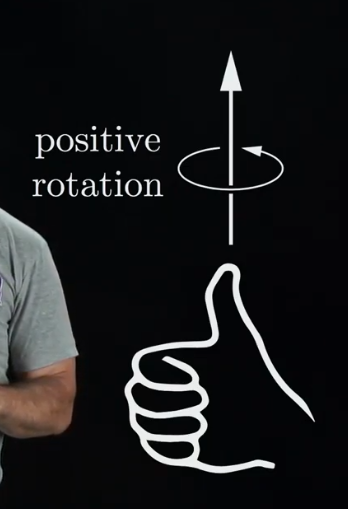
\includegraphics[width=0.5\textwidth]{postiveRotaion.png}
                      \caption{}
                      \label{fig:}
                  \end{figure}
    \section{Foundation of mobile robotics ch-2}
    \subsection{Degrees of freedom rigid body}
    \begin{itemize}
        \item \textbf{Configuration} - A specific position of the position of all points of robot
        \item \textbf{C-space} - The space of all configuration
        \item \textbf{degrees of freedom} - dimension of c space 
        \item Rigid body has 6 degrees of freedom
        \item dof - $\sum (freedom points) - no.of.constrains$
        \item $dof = m(N-1) - \sum_{i=1}^J c_i$ 
            \begin{figure}[htpb]
                        \centering
                        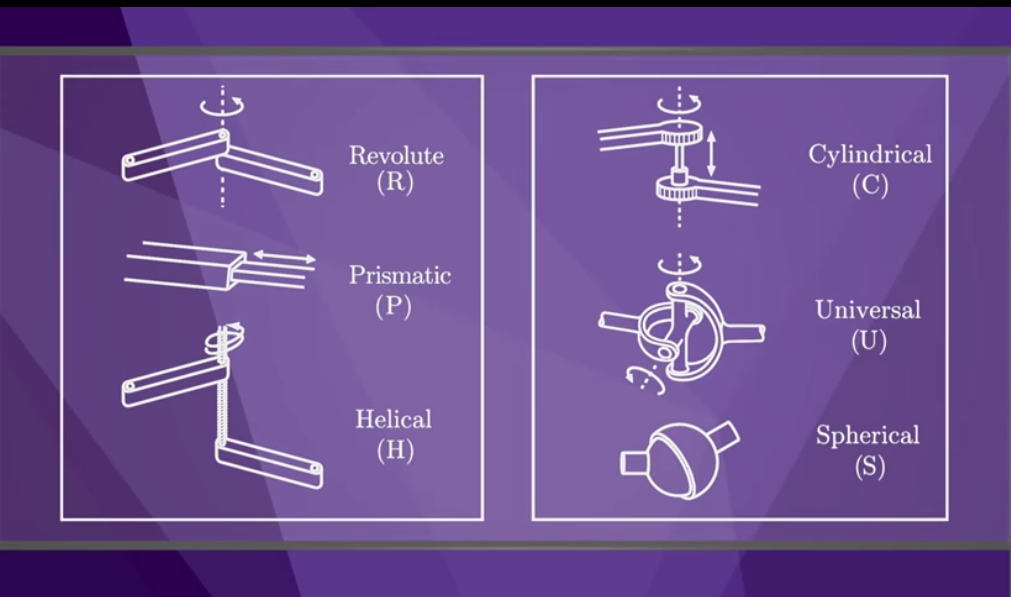
\includegraphics[width=0.8\textwidth]{joints.png}
                        \caption{}
                        \label{fig:}
                    \end{figure}
                    
    \end{itemize}
\end{document}
